%%%%%%%%%%%%%%%%%%%%%%%%%%%%%%%%%%%%%%%%%%%%%%%%%
%%%%%%%%%%%%%%%%%%%%%%%%%%%%%%%%%%%%%%%%%%%%%%%%%

\documentclass[12pt,a4paper]{scrartcl}

%%%%%%%%%%%%%%%%%%%%%%%%%%%%%%%%%%%%%%%%%%%%%%%%%
%%%%%%%%%%%%%%%%%%%%%%%%%%%%%%%%%%%%%%%%%%%%%%%%%

\usepackage[utf8]{inputenc}
\usepackage[english]{babel}
\usepackage[T1]{fontenc}

%%%%%%%%%%%%%%%%%%%%%%%%%%%%%%%%%%%%%%%%%%%%%%%%%
%%%%%%%%%%%%%%%%%%%%%%%%%%%%%%%%%%%%%%%%%%%%%%%%%

%\usepackage{ucs}
\usepackage{amsmath}
\usepackage{amssymb}

%%%%%%%%%%%%%%%%%%%%%%%%%%%%%%%%%%%%%%%%%%%%%%%%%
%%%%%%%%%%%%%%%%%%%%%%%%%%%%%%%%%%%%%%%%%%%%%%%%%

\usepackage{graphicx}
\usepackage{tabularx,colortbl}
\usepackage{capt-of}
\usepackage{booktabs}
\usepackage{hyperref}

%%%%%%%%%%%%%%%%%%%%%%%%%%%%%%%%%%%%%%%%%%%%%%%%%
%%%%%%%%%%%%%%%%%%%%%%%%%%%%%%%%%%%%%%%%%%%%%%%%%

\usepackage{pdflscape}
\usepackage{pdfpages}

%%%%%%%%%%%%%%%%%%%%%%%%%%%%%%%%%%%%%%%%%%%%%%%%%
%%%%%%%%%%%%%%%%%%%%%%%%%%%%%%%%%%%%%%%%%%%%%%%%%

\usepackage[group-separator={,}, group-minimum-digits=3]{siunitx}
\DeclareSIUnit\basepair{bp}
\DeclareSIUnit\byte{B}

%%%%%%%%%%%%%%%%%%%%%%%%%%%%%%%%%%%%%%%%%%%%%%%%%
%%%%%%%%%%%%%%%%%%%%%%%%%%%%%%%%%%%%%%%%%%%%%%%%%

\usepackage{biocon}
\newtaxon{strain}
\newtaxastyle{WithStrain}{\taxit{\taxonfirst{!genus!.}\taxon{ !epithet!}} str. \#\taxon{!strain!}}

\newanimal{Hd}{genus=Hybsibuis,epithet=dujardini}

%%%%%%%%%%%%%%%%%%%%%%%%%%%%%%%%%%%%%%%%%%%%%%%%%
%%%%%%%%%%%%%%%%%%%%%%%%%%%%%%%%%%%%%%%%%%%%%%%%%

\usepackage{enumitem}
\setlist[enumerate]{itemsep=0mm}

%%%%%%%%%%%%%%%%%%%%%%%%%%%%%%%%%%%%%%%%%%%%%%%%%
%%%%%%%%%%%%%%%%%%%%%%%%%%%%%%%%%%%%%%%%%%%%%%%%%

\usepackage{tabularx}
\usepackage[backend=biber]{biblatex}
\addbibresource{supplement.bib}
\usepackage{rotating}
\usepackage{cleveref}
\usepackage{listings}
\lstset{basicstyle=\ttfamily\footnotesize}

%%%%%%%%%%%%%%%%%%%%%%%%%%%%%%%%%%%%%%%%%%%%%%%%%
%%%%%%%%%%%%%%%%%%%%%%%%%%%%%%%%%%%%%%%%%%%%%%%%%

\title{\Large The genome of a tardigrade - \\\large Horizontal gene transfer or bacterial contamination?}
\author{\normalsize Felix Bemm, Clemens Weiß, Jörg Schultz, Frank Förster}
\date{}

%%%%%%%%%%%%%%%%%%%%%%%%%%%%%%%%%%%%%%%%%%%%%%%%%
%%%%%%%%%%%%%%%%%%%%%%%%%%%%%%%%%%%%%%%%%%%%%%%%%

\graphicspath{{./figures/}}
\DeclareGraphicsExtensions{.pdf,.PDF,.png,.PNG,.jpg,.JPG,.jpeg,.JPEG}

%%%%%%%%%%%%%%%%%%%%%%%%%%%%%%%%%%%%%%%%%%%%%%%%%
%%%%%%%%%%%%%%%%%%%%%%%%%%%%%%%%%%%%%%%%%%%%%%%%%

\begin{document}

\maketitle

\pagebreak

\section{Figures}

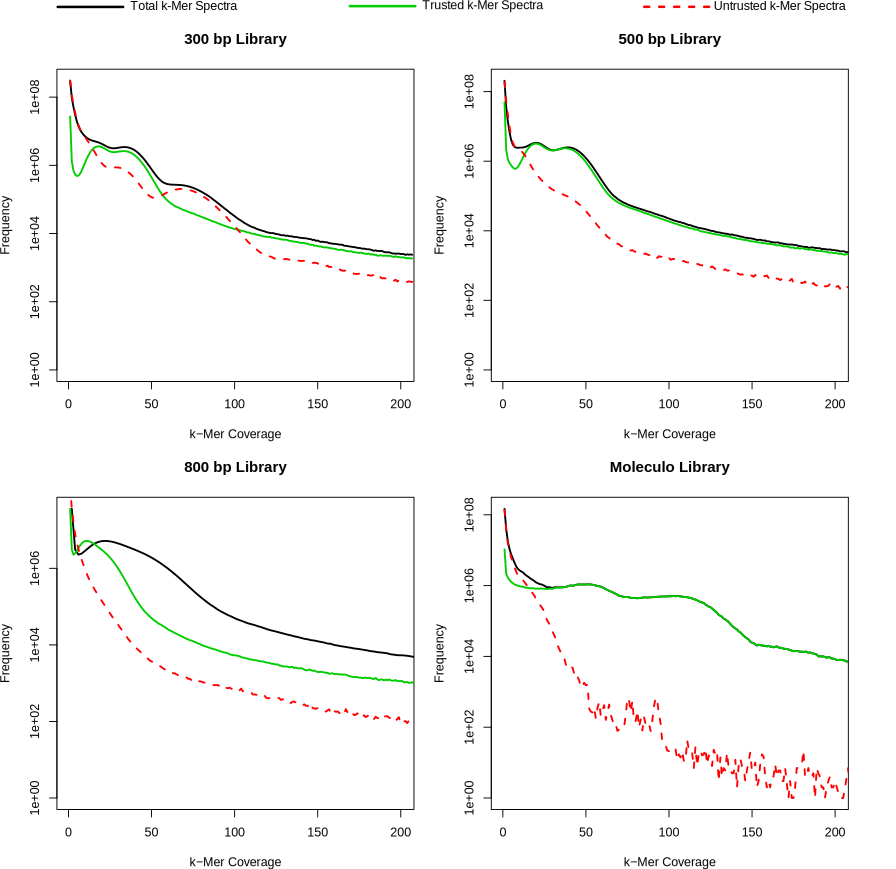
\includegraphics[width=1\textwidth]{supplementary_figure_1}
\captionof{figure}[k-Mer Analysis]{k-Mer Analysis}

\pagebreak

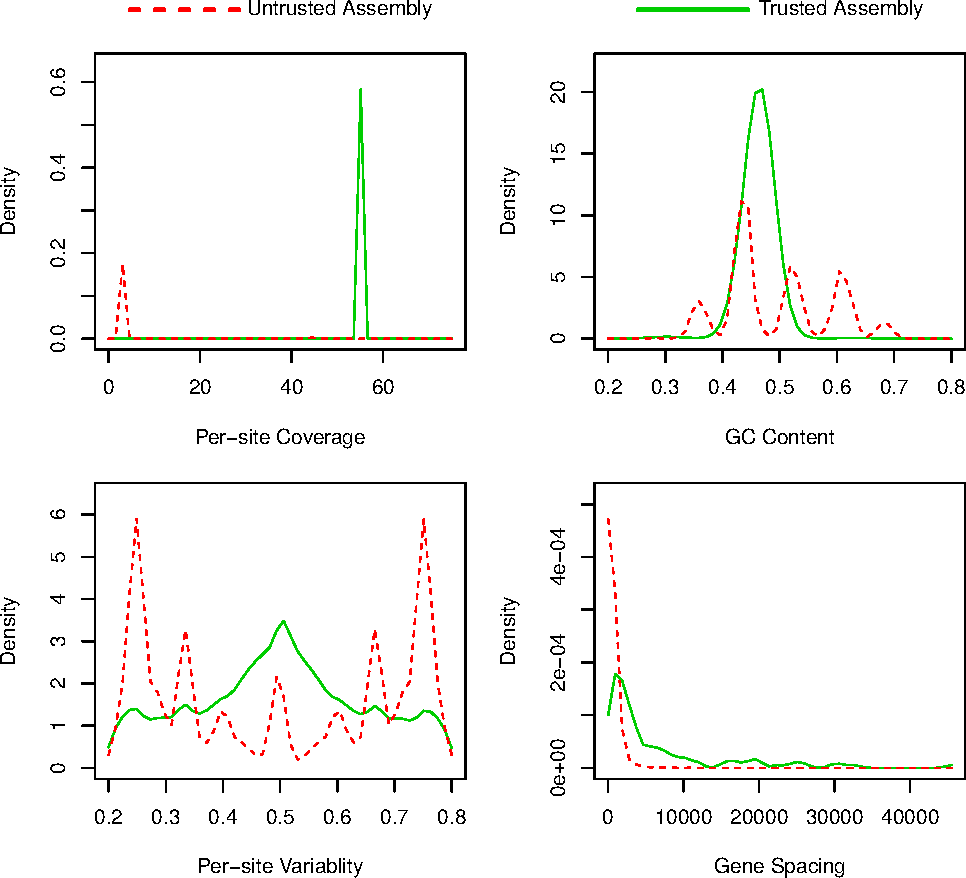
\includegraphics[width=1\textwidth]{supplementary_figure_2}
\captionof{figure}[Assembly Feature Comparisons]{Assembly Feature Comparisons}

\pagebreak

\includegraphics[width=1\textwidth]{supplementary_figure_3}
\captionof{figure}[Unknown Bacterial Genome]{Unknown Bacterial Genome}

\section{Methods}

\subsection*{Data set}
We used the data set provided by \textcite{Boothby2015} and downloaded the data from \url{http://weatherby.genetics.utah.edu/seq_transf/}. A complete list of the used input files are given in \cref{tab:inputdata}.

\begin{sidewaystable}
\centering
\captionof{table}{\label{tab:inputdata}Bla}
\begin{tabularx}{\linewidth}{>{\ttfamily\tiny}X>{\ttfamily\tiny}l>{\ttfamily\tiny}r*{2}{>{\ttfamily\tiny}l}}\toprule
Filename and location                                          & Modification time    & Size in Bytes     & MD5 check sum                    & MD5 check sum decompressed \\ \midrule
\href{http://weatherby.genetics.utah.edu/seq_transf/tg.genome.fsa.gz}{tg.genome.fsa.gz}
                                                               & 2015-11-25T01:34:44Z &    \num{72215266} & b8bd39390ef35dd43d1cda1ca6944d5a & 77be374d28b91232c0810cc4d3cd37b9 \\
\href{http://weatherby.genetics.utah.edu/seq_transf/tg.default.maker.proteins.final.fasta.gz}{tg.default.maker.proteins.final.fasta.gz}
                                                               & 2015-12-02T23:43:44Z &    \num{12359873} & 2de12e5d28d6dba121973db2071565d9 & 1ad17cfa9e6c26e552fa8048c6ee90af \\
\href{http://weatherby.genetics.utah.edu/seq_transf/short_reads/TG-300-SIPE_1_sequence.txt}{short\_reads/TG-300-SIPE\_1\_sequence.txt}
                                                               & 2015-11-30T21:48:51Z & \num{11526955725} & c16b5442c9893b6feaa3aa81a39eefcd & c16b5442c9893b6feaa3aa81a39eefcd \\
\href{http://weatherby.genetics.utah.edu/seq_transf/short_reads/TG-300-SIPE_2_sequence.txt.gz}{short\_reads/TG-300-SIPE\_2\_sequence.txt.gz}
                                                               & 2015-11-30T21:52:41Z &  \num{3920224257} & 3bea43d66d71926fb620966d281598c6 & bc8423d4fe4275863e0809445ffd21ce \\
\href{http://weatherby.genetics.utah.edu/seq_transf/short_reads/TG-500-SIPE_1_sequence.txt.gz}{short\_reads/TG-500-SIPE\_1\_sequence.txt.gz}
                                                               & 2015-12-01T05:32:05Z &  \num{2738243219} & da8b15d388961938584343f8926f7b24 & eee7363557ccb1fb0fa75ebe55ae7ee5 \\
\href{http://weatherby.genetics.utah.edu/seq_transf/short_reads/TG-500-SIPE_2_sequence.txt.gz}{short\_reads/TG-500-SIPE\_2\_sequence.txt.gz}
                                                               & 2015-12-01T05:35:15Z &  \num{2805269168} & aa8c2c345484b9464d272e0993d6968b & 325d74bbafd9b6019609e2fd33eca260 \\
\href{http://weatherby.genetics.utah.edu/seq_transf/short_reads/TG-800-SIPE_1_sequence.txt.gz}{short\_reads/TG-800-SIPE\_1\_sequence.txt.gz}
                                                               & 2015-12-01T05:36:55Z &  \num{2155735304} & 6e9cce1a27000ae2b4f87181a976df92 & a85568ef53979c367870eee6390f2ced \\
\href{http://weatherby.genetics.utah.edu/seq_transf/short_reads/TG-800-SIPE_2_sequence.txt.gz}{short\_reads/TG-800-SIPE\_2\_sequence.txt.gz}
                                                               & 2015-12-01T05:37:46Z &  \num{2058207374} & ccf097cf4f13bb5cbc5a8e002250093d & 4a4cc02c2f289d59c300810fb621eb28 \\
\href{http://weatherby.genetics.utah.edu/seq_transf/moleculo_reads/LR6000049-DNA_A01-LRAAD-01_LongRead.fastq.gz}{moleculo\_reads/LR6000049-DNA\_A01-LRAAD-01\_LongRead.fastq.gz}
                                                               & 2015-11-30T17:50:17Z &   \num{825877986} & 86e75544f2d6ef5185bae419bbd2a4b2 & bace73ed4750b33fc144e56c155454ab \\
\href{http://weatherby.genetics.utah.edu/seq_transf/moleculo_reads/LR6000049-DNA_A01-LRAAD-02_LongRead.fastq.gz}{moleculo\_reads/LR6000049-DNA\_A01-LRAAD-02\_LongRead.fastq.gz}
                                                               & 2015-11-30T17:51:34Z &   \num{835283315} & 4dea3e39a7a25059a6ebbd5588e845b2 & cb83c39f9a385f0b4fd1e507cfe40ff1 \\
\href{http://weatherby.genetics.utah.edu/seq_transf/moleculo_reads/LR6000049-DNA_A01-LRAAD-03_LongRead.fastq.gz}{moleculo\_reads/LR6000049-DNA\_A01-LRAAD-03\_LongRead.fastq.gz}
                                                               & 2015-11-30T17:52:51Z &   \num{847867943} & 16276b6ef8dea90721eb67ac21d616e6 & 51d4ce37668684b4aa25e061fb95b4ef \\
\href{http://weatherby.genetics.utah.edu/seq_transf/moleculo_reads/LR6000049-DNA_A01-LRAAD-04_LongRead.fastq.gz}{moleculo\_reads/LR6000049-DNA\_A01-LRAAD-04\_LongRead.fastq.gz}
                                                               & 2015-11-30T17:56:08Z &   \num{859746540} & 3364040445c7377c9323f82d98a2258c & dbe06ec4248199f416bb1d02ff1e65f5 \\
\href{http://weatherby.genetics.utah.edu/seq_transf/moleculo_reads/LR6000049-DNA_A01-LRAAD-05_LongRead.fastq.gz}{moleculo\_reads/LR6000049-DNA\_A01-LRAAD-05\_LongRead.fastq.gz}
                                                               & 2015-11-30T17:56:51Z &   \num{854266597} & 7995559df803ef0de0250f1bfac71f1a & 98d30f3ceb813d9f53c6df2ed1fa2239 \\
\end{tabularx}
\end{sidewaystable}

\subsection*{Programs}

\captionof{table}{\label{tab:programs}List of all programs including the version numbers and references to publications or websites used for the data processing and analysis}
\begin{tabularx}{\linewidth}{llX}\toprule
Programname & Version & Reference \\ \midrule
Allpath-LG  & v\,\textcolor{red}{XXXX} & \textcite{Gnerre2011, Ribeiro2012} \\
BEDTools    & v\,2.20.1 & \textcite{Quinlan2010} \\
bowtie2     & v\,2.2.2 & \textcite{Langmead2012} \\
bwa         & v\,0.7.10 & \textcite{Li2009,Li2010} \\
CGView      & v\,\textcolor{red}{XXXX} & \textcite{Grin2011} \textcolor{red}{???} \\
Falcon      & v\,\textcolor{red}{XXXX} & \url{https://github.com/PacificBiosciences/falcon} \\
GenemarkS   & v\,\textcolor{red}{XXXX} & \textcite{Besemer2001} \\
GenemarkET  & v\,\textcolor{red}{XXXX} & \textcite{Lomsadze2014} \\
Jellyfish   & v\,2.2.4  & \textcite{Marcais2011} \\
Perl        & v\,5.14.2  & \url{https://www.perl.org/} \\
\end{tabularx}

\subsection*{Trimming of the input data}

\subsection*{Estimation of the genomes size}

\subsection*{Counting and Filtering bases on kmers}

The kmers of all libraries where counted using the software jellyfish \parencite{Marcais2011}:

\begin{lstlisting}[language=bash]
# counting the kmers inside the trimmed sequence libraries
mkdir kmer
cd kmer
jellyfish count -t 32 -m 19 -s 30G -C \
   -o HD_gen.il_L300.trimmed_mer_19 \
   ../trimmed/HD_gen.il_L300.trimmed_P1.fastq \
   ../trimmed/HD_gen.il_L300.trimmed_P2.fastq
jellyfish count -t 32 -m 19 -s 30G -C \
   -o HD_gen.il_L500.trimmed_mer_19 \
   ../trimmed/HD_gen.il_L500.trimmed_P1.fastq \
   ../trimmed/HD_gen.il_L500.trimmed_P2.fastq
jellyfish count -t 32 -m 19 -s 30G -C \
   -o HD_gen.il_L800.trimmed_mer_19 \
   ../trimmed/HD_gen.il_L800.trimmed_P1.fastq \
   ../trimmed/HD_gen.il_L800.trimmed_P2.fastq
for i in $(find ../trimmed/ -name HD_gen.mo_L[12345]*.trimmed.formatted.fastq)
do
    jellyfish count -t 32 -m 19 -s 30G -C -o $(basename "$i" .fastq)_mer_19 "$i"
done

# merging of the moleculo hashes
jellyfish merge \
   -o HD_gen.mo_L1-5.trimmed.formatted_mer_19 \
   HD_gen.mo_L[12345].trimmed.formatted_mer_19
\end{lstlisting}

The resulting kmer hashes need to be dumped and converted to a hash
utilized later during the filtering step. This step and the following
required \SI{>200}{\giga\byte} of memory.

\begin{lstlisting}[language=bash]
cd kmer

# dumping the kmer hashes
for i in *_mer_19
do
   jellyfish dump --column --tab -o $(basename "$i").dump "$i"
done

# merging kmer hash information into a single perl hash
prepare_filter_fastq_by_valid_kmers.pl \
   --output kmer_hash.bin \
   --kmerlib 300=HD_gen.il_L300.trimmed_mer_19.dump \
   --kmerlib 500=HD_gen.il_L500.trimmed_mer_19.dump \
   --kmerlib 800=HD_gen.il_L800.trimmed_mer_19.dump \
   --kmerlib Moleculo=HD_gen.mo_L1-5.trimmed.formatted_mer_19.dump
\end{lstlisting}

The generated hash was used to filter individual libraries.

\begin{lstlisting}[language=bash]
mkdir kmer_filtered
cd kmer_filtered
../scripts/filter_fastq_by_valid_kmers_reduced.pl \
   --infile ../trimmed/HD_gen.il_L300.trimmed_P1.fastq,../trimmed/HD_gen.il_L300.trimmed_P2.fastq \
   --kmerhash ../kmer/kmers_hash.bin \
   --out HD_gen.il_L300.trimmed_P12.fastq.interleaved.filtered \
   --paired

../scripts/filter_fastq_by_valid_kmers_reduced.pl \
   --infile ../trimmed/HD_gen.il_L500.trimmed_P1.fastq,../trimmed/HD_gen.il_L500.trimmed_P2.fastq \
   --kmerhash ../kmer/kmers_hash.bin \
   --out HD_gen.il_L500.trimmed_P12.fastq.interleaved.filtered \
   --paired

../scripts/filter_fastq_by_valid_kmers_reduced.pl \
   --infile ../trimmed/HD_gen.il_L800.trimmed_P1.fastq,../trimmed/HD_gen.il_L800.trimmed_P2.fastq \
   --kmerhash ../kmer/kmers_hash.bin \
   --out HD_gen.il_L800.trimmed_P12.fastq.interleaved.filtered \
   --paired

for i in $(find ../trimmed/ -name HD_gen.mo_L[12345]*.trimmed.formatted.fastq)
do
   ../scripts/filter_fastq_by_valid_kmers_reduced.pl \
      --infile "$i" \
      --kmerhash ../kmer/kmers_hash.bin \
      --out $(basename "$i").filtered
done
\end{lstlisting}

The filtered data sets are classified as ``trusted'' or ``untrusted''
based on the ``trusted'' kmer content. Reads with at least
\SI{95}{\percent} ``trusted'' kmers content are called ``trusted''
while reads below that threshold are classified as ``untrusted''.

\begin{lstlisting}[language=bash]
pv HD_gen.il_L300.trimmed_P12.interleave.kmerfiltered.fastq | \
   perl -ne '
      unless (/percent_valid:([\d.]+)/) { die "Fehler"; }

      if ($1 < 0.95) {
        print STDERR $_, scalar <>,
                     scalar <>, scalar <>,
                     scalar <>, scalar <>,
                     scalar <>, scalar <>;
      } else {
        print $_,scalar <>,
              scalar <>, scalar <>,
              scalar <>, scalar <>,
              scalar <>, scalar <>;
      }' 2> HD_gen.il_L300.trimmed_P12.interleave.kmerfiltered.untrusted.fastq \
          > HD_gen.il_L300.trimmed_P12.interleave.kmerfiltered.trusted.fastq

pv HD_gen.il_L500.trimmed_P12.interleave.kmerfiltered.fastq | \
   perl -ne '
      unless (/percent_valid:([\d.]+)/) { die "Fehler"; }

      if ($1 < 0.95) {
        print STDERR $_, scalar <>,
                     scalar <>, scalar <>,
                     scalar <>, scalar <>,
                     scalar <>, scalar <>;
      } else {
        print $_,scalar <>,
              scalar <>, scalar <>,
              scalar <>, scalar <>,
              scalar <>, scalar <>;
      }' 2> HD_gen.il_L500.trimmed_P12.interleave.kmerfiltered.untrusted.fastq \
          > HD_gen.il_L500.trimmed_P12.interleave.kmerfiltered.trusted.fastq

pv HD_gen.il_L800.trimmed_P12.interleave.kmerfiltered.fastq | \
   perl -ne '
      unless (/percent_valid:([\d.]+)/) { die "Fehler"; }

      if ($1 < 0.95) {
        print STDERR $_, scalar <>,
                     scalar <>, scalar <>,
                     scalar <>, scalar <>,
                     scalar <>, scalar <>;
      } else {
        print $_,scalar <>,
              scalar <>, scalar <>,
              scalar <>, scalar <>,
              scalar <>, scalar <>;
      }' 2> HD_gen.il_L800.trimmed_P12.interleave.kmerfiltered.untrusted.fastq \
          > HD_gen.il_L800.trimmed_P12.interleave.kmerfiltered.trusted.fastq
\end{lstlisting}

\subsection*{Long Read Assembly}

Falcon

\subsection*{Assembly Annotation}

GeneMark-S and GeneMark-ES
CGView -> Visualizatin

\subsection*{Assembly Comparison}

GC Sliding Windows ?
Mapping Coverage ?
Per-site Variability ?
sm-Packages to compare distributions

\printbibliography

\end{document}
